\documentclass[a4paper,12pt]{article}
\usepackage[utf8]{inputenc}
\usepackage[spanish]{babel}
\usepackage[T1]{fontenc}
\usepackage[nofontinfo]{lucidabr}
\usepackage{calc, graphicx}
\usepackage[format=hang, font=small, labelfont=bf, labelsep=endash, width=.9\textwidth]{caption}
\usepackage[listofformat=subsimple, format=hang, labelfont=footnotesize, textfont={it, footnotesize}]{subfig}
\title{Figuras elaboradas con MetaPost}
\author{José Ramón Gisbert Valls}
\newcommand\texto{Este manual está destinado a todo aquel usuario interesado en la representación de señales eléctricas en el contexto que se ha expuesto anteriormente en el libro. En concreto, puede ser de especial interés para aquellos usuarios que deseen representar el espectro en frecuencia de una señal eléctrica en tiempo real, de forma que al mismo tiempo pueda visualizarse la señal correspondiente a dicho espectro.}
\begin{document}


\maketitle{}

\begin{abstract}
	Este documento me permite seguir el aspecto que muestran las figuras elaboradas en MetaPost para su inclusión en la memoria al ritmo en el que las voy desarrollando.
\end{abstract}

\listoffigures

\begin{figure}
	\begin{center}
		\includegraphics{gis-pfc-part1-01.mps}
	\end{center}
	\caption[Sistema digital de medida]{Esquema que muestra las distintas unidades funcionales de un sistema digital de medida.}
	\label{fig:digmeasstm}
\end{figure}

\begin{figure}
	\begin{center}
		\includegraphics{gis-pfc-ch1-01.mps}
	\end{center}
	\caption[Subsistema para la interacción con el medio]{Subsistema para la interacción con el medio.}
	\label{fig:submedium}
\end{figure}

\begin{figure}
	\begin{center}
		\includegraphics[angle=90]{gis-pfc-ch1-02.mps}
	\end{center}
	\caption[Circuito acondicionador de la sección de transmisión]{Circuito acondicionador de la sección de transmisión.}
	\label{fig:txaconditioner}
\end{figure}

\begin{figure}
	\begin{center}
		\includegraphics{gis-pfc-ch1-03.mps}
	\end{center}
	\caption[Señal a la salida del amplificador \textsc{ne5534}, $u(t)$]{Señal generada por el acondicionador de transmisión medida a la salida del amplificador \textsc{ne5534}, $u(t)$.}
	\label{fig:txacvo}
\end{figure}

\clearpage

\begin{figure}
	\begin{center}
		\includegraphics{gis-pfc-ch1-04.mps}
	\end{center}
	\caption[Pulso acústico generado por el transductor]{Pulso acústico generado por el transductor cuando se alimenta con un pulso rectangular.}
	\label{fig:pulse}
\end{figure}

\begin{figure}
	\begin{center}
		\includegraphics{gis-pfc-ch2-01.mps}
	\end{center}
	\caption[Subsistema de adquisición]{Subsistema de adquisición.}
	\label{fig:subacqui}
\end{figure}

\begin{figure}
	\begin{center}
		\includegraphics{gis-pfc-ch2-02.mps}
	\end{center}
	\caption[Ejemplo de configuración de terminación]{Figura que muestra el modo de terminación sencillo. La entrada superior del amplificador de instrumentación se conecta al puerto 9 y la entrada inferior se conecta a masa.}
	\label{fig:termmodes}
\end{figure}

\begin{figure}
	\begin{center}
		\includegraphics{gis-pfc-ch2-03.mps}
	\end{center}
	\caption[Conector etiquetado como \emph{analog}]{Conector etiquetado como \emph{analog}.}
	\label{fig:analog}
\end{figure}

\clearpage

\begin{figure}
	\begin{center}
		\includegraphics{gis-pfc-ch2-04.mps}
	\end{center}
	\caption[Conector etiquetado como \emph{digital}]{Conector etiquetado como \emph{digital}.}
	\label{fig:digital}
\end{figure}

\begin{figure}
	\begin{center}
		\includegraphics{gis-pfc-ch3-01.mps}
	\end{center}
	\caption[Subsistema de control y presentación]{Subsistema de control y presentación.}
	\label{sub:control}
\end{figure}

\begin{figure}
	\begin{center}
		\includegraphics{gis-pfc-ch3-02.mps}
	\end{center}
	\caption[Fragmento de señal adquirido por el osciloscopio en el espacio de una ventana de adquisición]{Fragmento de señal adquirido por el osciloscopio en el espacio de una ventana de adquisición. En esta figura se ha representado también la duración de la ventana temporal del osciloscopio, pudiendo observarse que información se descarta. También se indica el instante en el que se inicia una nueva instancia del proceso de adquisición, de lo que puede deducirse que información se pierde entre instancias. Los cortes de la señal con el nivel de disparo también están representados.}
	\label{fig:freesignal}
\end{figure}

\begin{figure}
	\begin{center}
		\includegraphics{gis-pfc-ch3-03.mps}
	\end{center}
	\caption[Modo de funcionamiento disparado]{Modo de funcionamiento disparado. La representación se centra en el corte central (veáse la figura anterior).}
	\label{fig:digtrigosc}
\end{figure}

\clearpage

\begin{figure}
	\begin{center}
		\includegraphics{gis-pfc-ch3-04.mps}
	\end{center}
	\caption[Fragmentos de señal ordenados según llegan al osciloscopio]{Fragmentos de señal adquiridos por el osciloscopio en el modo continuo de funcionamiento. Se empieza a monitorizar la señal en $t_0$, los instantes posteriores están separados entre sí una ventana de adquisición. Debe recordarse que en el modo continuo se emplea con señales <<lentas>> por lo que la separación entre instancias es de adquisición es prácticamente nula en comparación con el periodo de la señal.}
	\label{fig:freesignalcont}
\end{figure}

\begin{figure}
	\begin{center}
		\includegraphics{gis-pfc-ch3-05.mps}
	\end{center}
	\caption[Modo de funcionamiento continuo del osciloscopio]{Modo de funcionamiento continuo. Puede observarse como el fragmento de señal representado en primer lugar es desplazado a la derecha para poder insertar el nuevo fragmento de señal. Obviamente, en $t_0$ la pantalla del osciloscopio estará en blanco.}
	\label{fig:digcontosc}
\end{figure}

\begin{figure}
	\begin{center}
		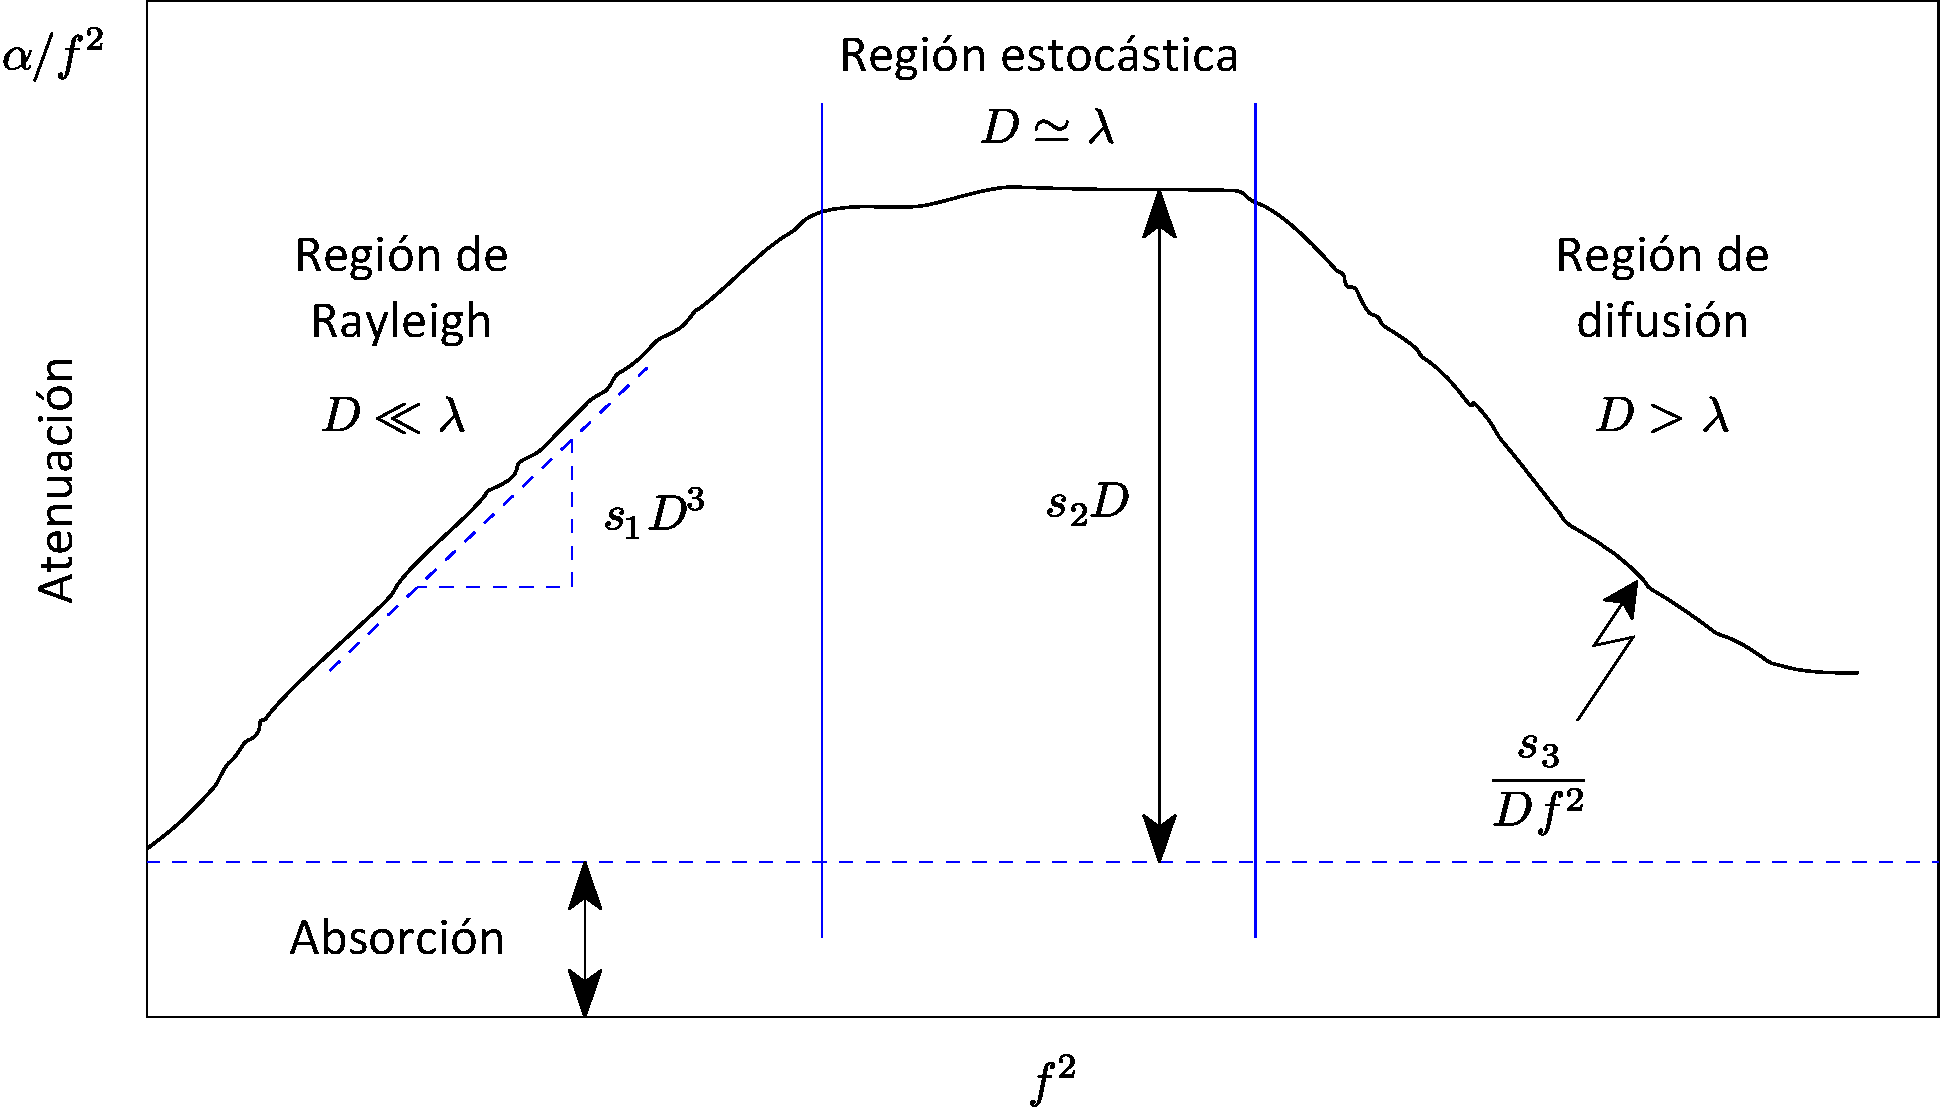
\includegraphics{gis-pfc-ch3-06.mps}
	\end{center}
	\caption[Modo de funcionamiento continuo]{La ventana temporal tiene, en este ejemplo, una duración de cinco ventanas de adquisición. Al llegar el osciloscopio el sexto fragmento de señal, la representación avanza a la derecha, retirándose el primer fragmento representado para dar lugar al fragmento obtenido recientemente.}
	\label{fig:digcontosccont}
\end{figure}

\begin{figure}
	\begin{center}
		\includegraphics{gis-pfc-ch3-07.mps}
	\end{center}
	\caption[Componentes de la \textsc{dat}]{Componentes de la \textsc{dat}.}
	\label{fig:dat}
\end{figure}

\clearpage

\begin{figure}
	\begin{center}
		\includegraphics{gis-pfc-ch3-08.mps}
	\end{center}
	\caption[Tipos de objeto dispositivo]{Tipos de objeto dispositivo.}
	\label{fig:devobject}
\end{figure}

\begin{figure}
	\begin{center}
		\includegraphics{gis-pfc-ch5-01.mps}
	\end{center}
	\caption[Campo generado por un transductor]{Campo generado por un transductor.}
	\label{fig:field}
\end{figure}

\begin{figure}
	\begin{center}
		\includegraphics{gis-pfc-ch5-02.mps}
	\end{center}
	\caption[\textsc{endus} por transmisión]{\textsc{endus} por transmisión.}
	\label{fig:transmission}
\end{figure}

\begin{figure}
	\begin{center}
		\includegraphics{gis-pfc-ch5-03.mps}
	\end{center}
	\caption[\textsc{endus} por pulso"=eco]{\textsc{endus} por pulso"=eco.}
	\label{fig:echo}
\end{figure}

\clearpage

\begin{figure}
	\begin{center}
		\includegraphics{gis-pfc-ch5-04.mps}
	\end{center}
	\caption[Modelo de emisión"=transmisión]{Diagrama de bloques que muestra el modelo empleado para calcular la respuesta al impulso de emisión"=recepción.}
	\label{fig:model}
\end{figure}

\begin{figure}
	\begin{center}
		\includegraphics{gis-pfc-ch5-05.mps}
	\end{center}
	\caption[Modelo de matriz de pequeños reflectores]{Modelo de matriz de pequeños reflectores.}
	\label{fig:matrix}
\end{figure}

\begin{figure}
	\begin{center}
		\includegraphics{gis-pfc-ch5-07.mps}
	\end{center}
	\caption[Parámetros del banco de filtros]{Representación esquematizada en el que se identifican los parámetros de la \textsc{fft} y su relación con respecto a la señal.}
	\label{fig:filter}
\end{figure}
% 
% \newsavebox{\txbox}
% \sbox{\txbox}{\includegraphics[draft=true]{gis-pfc-ch5-07.mps}}
% \newsavebox{\gxbox}
% \sbox{\gxbox}{\includegraphics[draft=true]{palm-trees-01.mps}}
% \newlength{\txwidth}
% \setlength{\txwidth}{4pt + \wd\txbox - \wd\gxbox}
% 
% \begin{figure}
% 	\begin{center}
% 		\hspace*{\txwidth}\includegraphics{palm-trees-01.mps}
% 	\end{center}
% 	\caption[Ejemplo de gráfica]{Ejemplo de gráfica con dimensiones de 120 mm de largo por 90 mm de alto.}
% 	\label{fig:palmone}
% \end{figure}

\end{document}
